\subsubsection{Modelo: Servicios de comunicación de estado}

El sistema de comunicación necesita mantener la conexión \gls{tcp} para poder tener control del dispositivo desde servidor.
La mayoría de protocolos resuelven este problema enviando un paquete de información de estado cada cierto tiempo si el sistema detecta que no se está enviando información.
El protocolo de nivel inferior utilizado, en el caso propio de este protocolo siendo \gls{tcp}, incluye en su capa de control un modelo de establecer \gls{keepalive}, este sistema cuenta con el problema de su poca configuración en determinados dispositivos y cuenta con un tiempo entre paquetes relativamente alto, del orden de dos horas por defecto en el kernel estandar de Linux. Algunas implementaciones, permiten configurar este parámetro no siendo una configuración sencilla de aplicar a nivel de aplicación. Por este motivo es necesario crear un servicio de control de estado.

Como puede observarse en la figura \ref{fig:modelo_servicios_comunicacion_estado_classes}, contamos con la clase \textit{StatusService} que a su vez implementa la clase del modelo anterior \textit{Service}. A su vez, vemos las clases \textit{Ping} y \textit{Pong} que implementan la clase \textit{StatusService}.

El funcionamiento de este modelo es relativamente sencillo. Si el sistema no detecta actividad en ninguna de las dos direcciones de comunicación, tanto de cliente a servidor como de servidor a cliente en un tiempo determinado, enviará un paquete \textit{Ping}, respondiendo a su llegada el destinatario con un paquete \textit{Pong}.

\begin{figure}
	\centering
    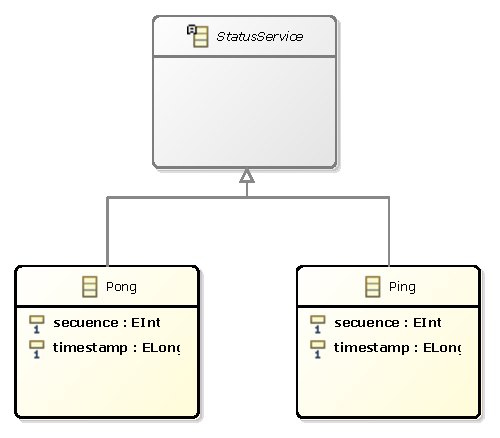
\includegraphics[height=0.3\textheight]{images/models/communicationstatus_class_diagram.pdf}
    \captionmodeloclase{Servicios de comunicación - Estado de conexión.}
    \label{fig:modelo_servicios_comunicacion_estado_classes}
\end{figure}

\clearpage
